The INDI discovery systems is currently being used for chat and multimedia applications in the Naval Research Lab \cite{Macker2010a, Dean2011}.  It provides low level modes for service discovery in mobile networked environments and provides interfaces for allowing applications to use this functionality to enable end-to-end connectivity.  In this section, we describe ProtoSD, which is the operating and service visualization environment for INDI and outline some of the applications that are INDI is motivated by. 

Proto Service Discovery (ProtoSD) is a toolkit that provides a single homogeneous toolkit for running both the mDNS and INDI discovery systems.   ProtoSD has a: command-line interface modeled using Apple's ``mdns'' command line tool for Bonjour; file-based interface for allowing third party applications to be integrated; and a Web-based interface for dynamic visual representation of the discovered services through a conventional Web browser.   The file interface and Web interface are the two most commonly used.  For the file interface, ProtoSD can optionally be used to generate ``.services'' files,  providing a simple file-based API for other applications to interface with e.g. we are currently using this with Python to read the ``.services'' file and provide a TV channel for incoming videos.  It also allows a single sink application to read services from multiple sources on a shared file system, which enables service browsing in CORE .  Our two main usages therefore are:

\begin{description}
\item [Private Service Browser:] by running the ProtoSD Web component locally and  browsing the network using the command line with a ``-g'' flag, ProtoSD enables the back-end Web server to provide a dynamic updated view of the services.  
\item [CORE Service Browser:] using CORE's shared file system, it is possible to use ProtoSD to show the services being discovered on all CORE nodes simultaneously using one browser.
\end{description}

For private browsing, ProtoSD passes service discovery and removal announcements directly to the command line or Web browser component for visualization, whilst for CORE, the ProtoSD file interface is used to bridge between CORE and the host Web browser.    Each CORE node stores its discovered services  in ``/tmp'' within ``.services'' files (named after their node name and network interface). The host scans this directory for write updates and loads all files simultaneously for rendering in a Web browser. Since the CORE nodes are not easily connected to the host, this simple shared file based mechanism provides a convenient way of visualizing the services without needing to reconfigure the default set up of CORE.   Using this approach, one can give a global view the services dynamically as and when services are advertised and removed from the network.  All of the emulations described in Section \ref{sec:results} used ProtoSD to visualize the output as the emulations were taking place.  This also provides a quick-look verification mechanism for ensuring the runs were operating normally and thus expedited the process.   

\begin{figure}[h!]
\centering
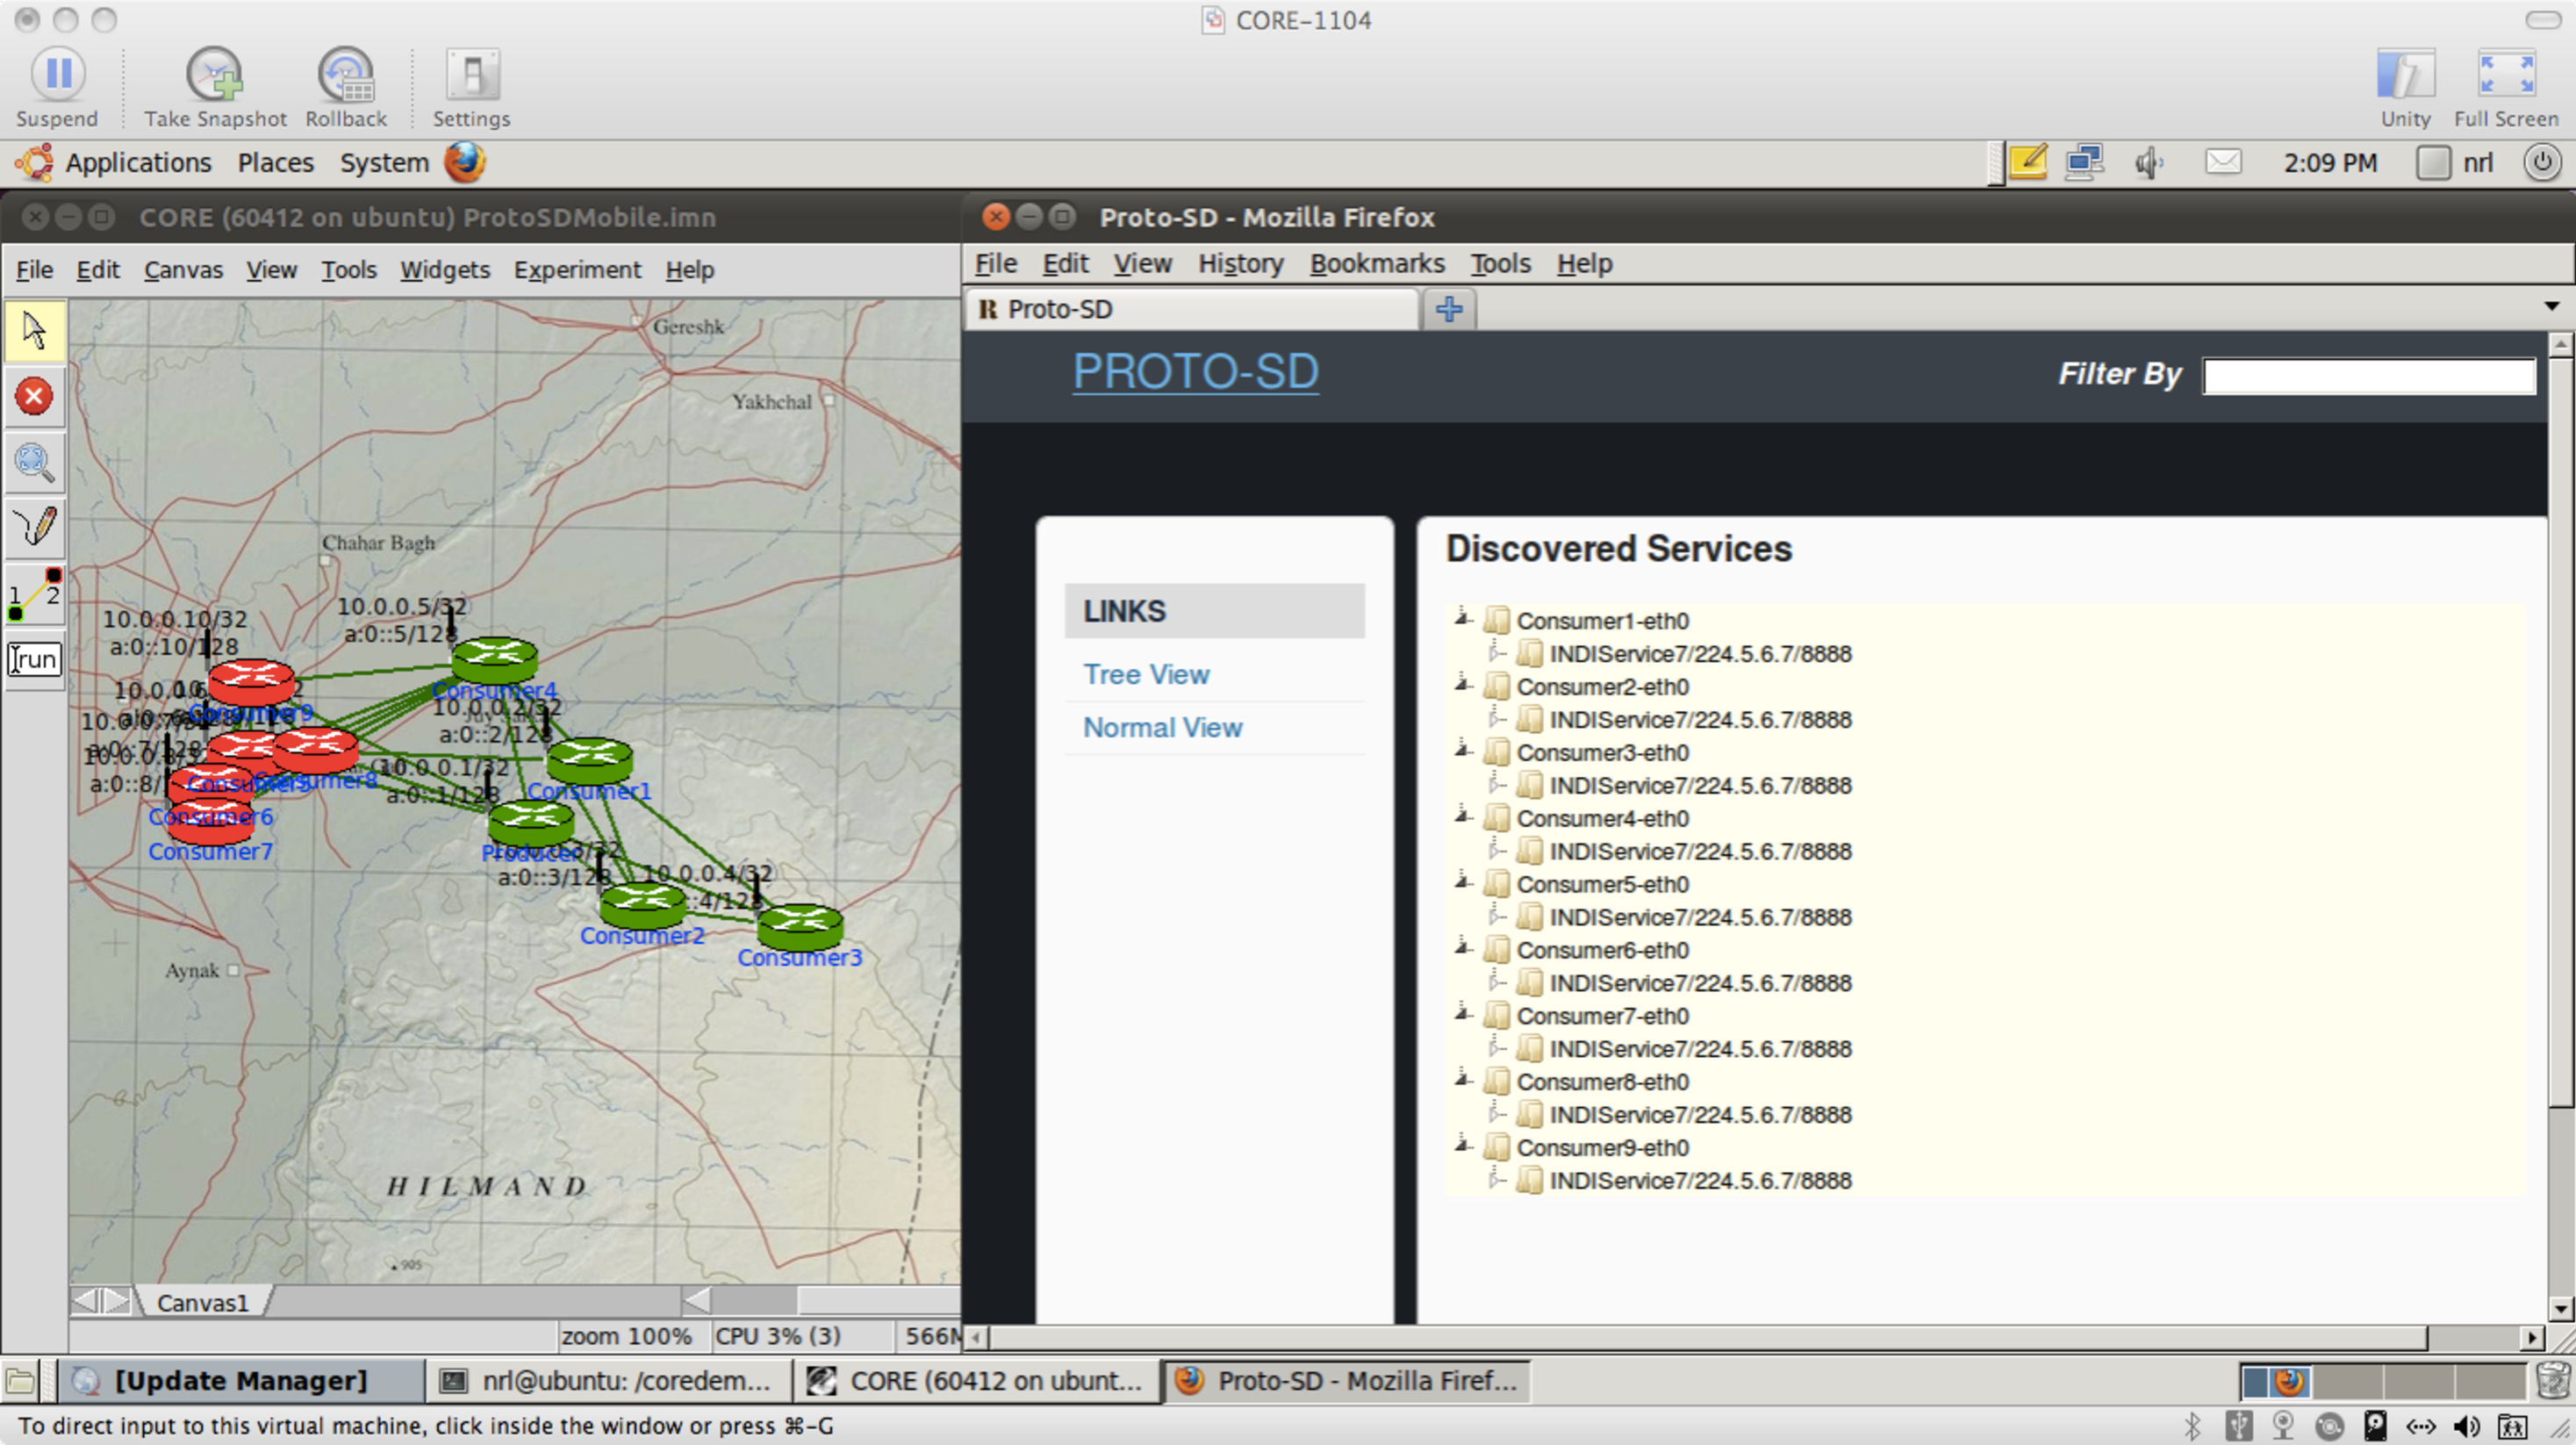
\includegraphics[width=5.5in]{ProtoSDCore.pdf}
\caption{ProtoSD running in CORE showing the services discovered during one mobile emulation for the INDI discovery system.} 
\label{indi:protosdcore}
\end{figure}

On the right hand side of Figure \ref{indi:protosdcore}, we show a screenshot of the ProtoSD Web interface, displaying the services it has discovered from each consumer in a CORE emulation in a tree view.  ProtoSD uses a Java-based lightweight Web server framework, called Restless\footnote{Restless was developed by Andrew Harrison, now working for  the Carefx Corporation but not yet released publicly}, for exposing the backend services.   Restless is a simple HTTP 1.0 compliant Web server that is capable of delivery multiple types of data efficiently and providers virtual endpoints for representing services using REST facilitating the Create, Read, Update and Delete (CRUD) style of operations.  To enable dynamic updates, ProtoSD uses a client-side JQuery component \footnote{http://jquery.com/}  that queries the server using an AJAX asynchronous HTTP GET to return service advertisement updates as and when new services are available. In this way, the browser updates immediately upon discovery of a new service (i.e. uses the COMET style\footnote{http://en.wikipedia.org/wiki/Comet\_(programming)} of server callback). By exposing two independent endpoints for fetching a JSON or HTML data structure from the server, it can render  using either a JsTree\footnote{http://www.jstree.com/} JQuery tree structure or HTML, for displaying to the users. Using the ``search'' textfield at the top right allows pruning of this list to match only the provided string.  

\begin{figure}[h!]
\centering
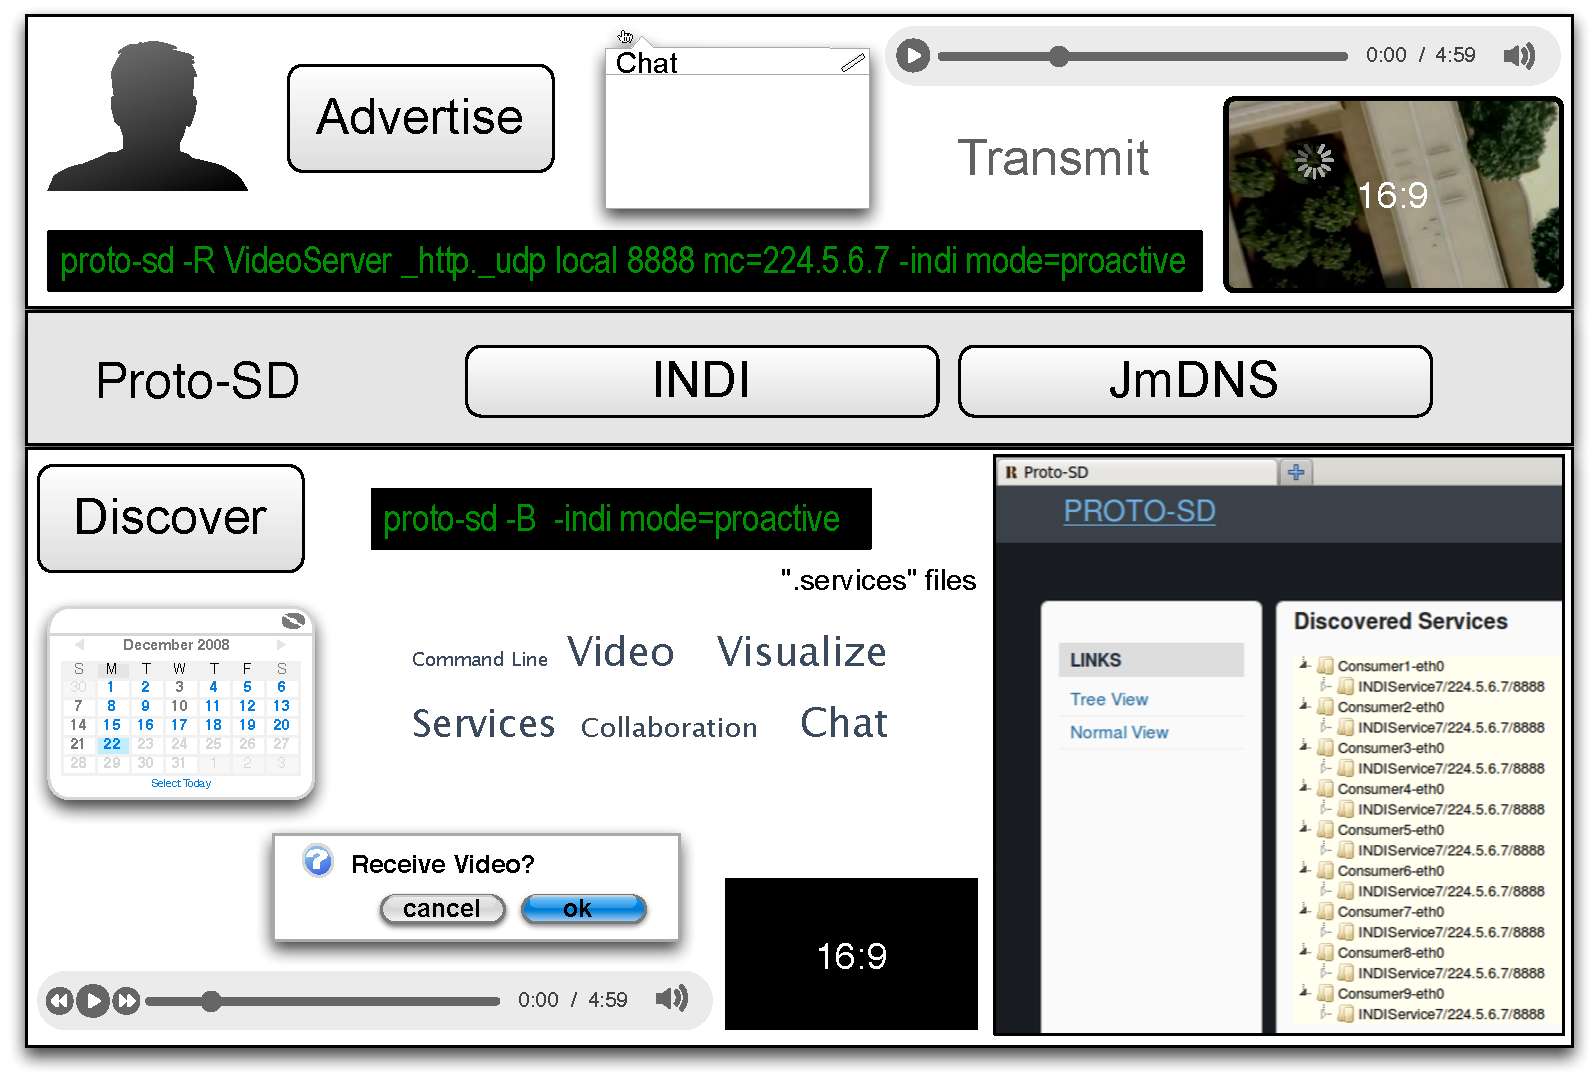
\includegraphics[width=5.5in]{ProtoSD.pdf}
\caption{An overview of ProtoSD showing the interfaces by which services are advertised and how services can be discovered and visualized.   We also show the kinds of applications ProtoSD has already been implemented with.} 
\label{indi:protosd}
\end{figure}

Figure \ref{indi:protosd} shows an overview of the various components involved in advertising and discovering using ProtoSD and some of the application use cases.   ProtoSD has been used as a private browser for discovering multimedia (video and audio) streams and providing an interface for allowing clients to connect to them using video toolkits (e.g. VLC\footnote{http://www.videolan.org/vlc/}).  For some applications, the Web GUI also provides an off-the-shelf solution for exposing management information about the participants in the network.  For example, for an XMPP multi-user chat (MUC) session, the ProtoSD browser can be used to provide a similar mechanism to what centralized XMPP management servers provide for administrators. Using OpenFire\footnote{http://www.igniterealtime.org/projects/openfire/}, an administrator can view the current MUC rooms created by users that are currently connected to this server.   For ProtoSD, the MUC rooms that are created by its users also appear as adverts on the multicast network and are consequently discovered by ProtoSD and listed through the Web GUI accordingly.  ProtoSD and INDI have already been used for this purpose by integrating with the XOP\cite{xop2010} serverless XMPP chat system on a MANET. 

